\section{Theorie}
\label{sec:Theorie}

Greifen an der Oberfläche eines Körpers Kräfte an, kann es zu Gestaltsänderungen des Körpers kommen.
Ein Beispiel für eine solche Verformung ist die Längenänderung eines Körpers unter dem Einfluss einer
zur Oberfläche senkrecht wirkenden Normalspannung $\sigma$. Ist die Längenänderung $\Delta L$ dabei hinreichend klein
gegenüber der Ausgangslänge $L$, so lässt sich die Verformung gemäß dem Hookschen Gesetz nach
\begin{equation}
    \sigma = E \frac{\Delta L}{L}
    \label{eq:hooke}
\end{equation}
beschreiben. Der Proportionalitätsfaktor $E$ ist dabei der Elastizitätsmodul. Dieser ist eine in der Werkstofftechnik
wichtige Materialkonstante.
Kann die Längenänderung zuverlässig gemessen werden, kann der Elastizizätsmodul direkt aus der Dehnung eines Körpers bestimmt werden.
In diesem Versuch wird der Elastizitätsmodul allerdings durch eine andere Art der Verformung bestimmt, nämlich durch die Biegung:
\begin{figure}[H]
    \centering
    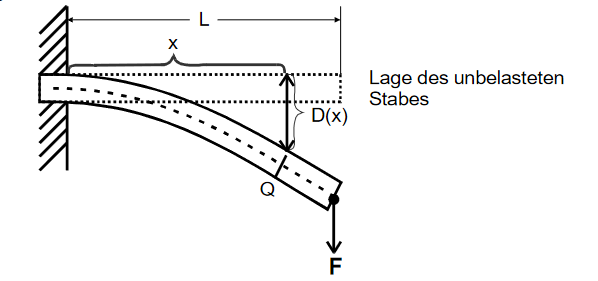
\includegraphics[width=0.7\textwidth]{assets/biegung.png}
    \caption{Biegung eines einseitig eingespannten Stabes \cite{V103}.}
    \label{fig:biegung}
\end{figure}
\noindent Wird ein Stab wie in \autoref{fig:biegung} dargestellt einer Kraft $F$ ausgesetzt, bewirkt die Kraft an der Stelle $x$ ein äußeres Drehmoment
\begin{equation}
    M_{F} = F (L-x) .
\end{equation}
Durch die Verformung treten innerhalb des Stabes Spannungen auf. Der obere Teil des Stabes wird dabei gedehnt, während der untere Teil gestaucht wird.
Dazwischen liegt eine Fläche, deren Länge unverändert bleibt, die sogenannte neutrale Faser. Die Zug- und Druckspannungen wirken in entgegengesetzte Richtungen,
sie erzeugen somit widerum ein inneres Drehmoment
\begin{equation}
    M_{\sigma} = \int_Q y \sigma(y) dq
\end{equation}
im Stab. $Q$ ist dabei die Querschnittsfläche des Stabes, $y$ der Abstand des Flächenelementes $dq$ zur neutralen Faser und $\sigma(y)$ die durch die Verformung hervorgerufene
Normalspannung.
$M_F$ und $M_\sigma$ sind entgegengesetzt, sodass es bei
\begin{equation}
    M_F = M_{\sigma}
\end{equation} 
zu einem Gleichgewichtszustand mit einer endlichen Durchbiegung $D$ kommt.
Die Spannungen $\sigma(y)$ können durch das Hooksche Gesetz ausgedrückt werden, sodass sich nach einigen Umformungen die Gleichung
\begin{equation}
    D(x) = \frac{F}{2EI} \left( L x^2 - \frac{x^3}{3}\right)
    \label{eq:einsietige_Biegung}
\end{equation} 
für die Durchbiegung ergibt.Der Term $I = \int_Q y^2 dq$ ist dabei das Flächenträgheitsmoment.
Dieses ist abhängig vom Querschnitt des Stabes. Es lässt sich berechenen nach
\begin{equation}
    I = Q \frac{b^2}{12}
    \label{eq:traegheitsmoment_quadratisch}
\end{equation}
für quadratische Stäbe (wobei $b$ die Kantenlänge ist), bzw nach
\begin{equation}
    I = \frac{Q}{4} R^2
    \label{eq:traegheitsmoment_rund}
\end{equation}
für runde Stäbe (mit dem Radius $R$).
\begin{figure}[H]
    \centering
    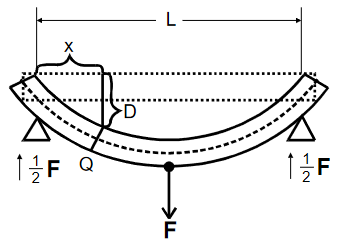
\includegraphics[width=0.7\textwidth]{assets/biegung_2.png}
    \caption{Biegung eines beidseitig eingespannten Stabes [1].}
    \label{fig:biegung_2}
\end{figure}
\noindent Bei einem beidseitig eingespannten Stab, bei dem die Kraft in der Mitte des Stabes angreift (siehe \autoref{fig:biegung_2}) ergeben sich die Gleichungen
\begin{align}
    & D(x) = \frac{F}{48EI} \left(3 L^2 x -4 x^3\right) & \mathrm{für} \; 0 \geq x \geq \frac{L}{2} \\
    & D(x) = \frac{F}{48EI} \left(4x^3 - 12 L x^2 + 9L^2 x - L^3\right) & \mathrm{für} \; \frac{L}{2} \geq x \geq L
    \label{eq:beidseitige_biegung}
\end{align}
für die Durchbiegung.